\documentclass{article}

\usepackage[utf8]{inputenc}
\usepackage{lmodern}
\usepackage{amsmath}
\usepackage{enumitem}% http://ctan.org/pkg/enumitem
\usepackage[ngerman]{babel}
\usepackage[ngerman]{translator} % Weitere Übersetzungen
\usepackage{graphicx}
\usepackage{fancyhdr}
\usepackage{roboto}
\usepackage{sectsty}
\usepackage{lastpage}
\usepackage{layout}
\usepackage{listings}
\usepackage{makecell}
\usepackage{tabularx}
\usepackage[table]{xcolor}
\usepackage{tikz}
\usepackage{array}
\usepackage{lipsum}
\usepackage{multirow}
\usepackage{float}
\usepackage{titlesec}
\usepackage{caption}
\usepackage{hyperref}
\usepackage{geometry}            % Dient zur Interface dimensionierung
\usepackage{pdflscape}           % bessere Lesbarkeit des PDF Dokuments
\usepackage{typearea}  % loaded automatically if using KOMA-Script class
\usepackage{etoolbox}
\usepackage{pgfgantt}

\patchcmd{\thebibliography}{\chapter*}{\section*}{}{}
\lstset{language=ruby}

\hypersetup{%
    colorlinks=false,% hyperlinks will be black
    pdfborderstyle={/S/U/W 0}% border style will be underline of width 1pt
}

\titleformat{\chapter}{\Huge\bfseries\sffamily}{\thechapter}{1em}{\Huge}

%Tabellen Caption links orientiert
\captionsetup[table]{skip=0pt,singlelinecheck=off}

%Weitere Spalten typen
\newcolumntype{L}[1]{>{\raggedright\let\newline\\\arraybackslash\hspace{0pt}}m{#1}}
\newcolumntype{C}[1]{>{\centering\let\newline\\\arraybackslash\hspace{0pt}}m{#1}}
\newcolumntype{R}[1]{>{\raggedleft\let\newline\\\arraybackslash\hspace{0pt}}m{#1}}

%Seitenformatierung anpassen
\textwidth=400pt
\textheight=600pt
\oddsidemargin=25pt
\fancypagestyle{plain}{}
\pagestyle{fancy}
\setlength{\parindent}{0pt}

%Sans seriff Font
\allsectionsfont{\sffamily}

%Header höhe anpassen
\setlength\headheight{33pt}
%Bilderpfad
\graphicspath{{bilder/}}
%Header und Footer
\fancyhf{}
\lfoot{\today}
\rfoot{Seite \thepage \hspace{1pt} von \pageref{LastPage}}
\lhead{Symmetrische und Asymmetrische Verschlüsselungsarten}
\rhead{Sylvain Gilgen}

%Weiteres
\definecolor{puzzleblue}{RGB}{30,90,150}
\author{Sylvain}
\title{IPA}
\include{codestyle}

\begin{document}
\huge \textbf{Symmetrische und Asymmetrische Verschlüsselungsarten} \normalsize
\section*{Symmetrische Verschlüsselung}
Bei symmetrischen Verschlüsselungsverfahren wird ein Schlüssel verwendet zum ver- und entschlüsseln. Aus diesem Grund ist es ein symmetrisches Verfahren.

Symmetrische Verschlüsselungsverfahren:

\begin{itemize}
    \item AES (Advanced Encryption Standard)
    \item DES (Data Encryption Standard)
    \item Triple-DES
    \item IDEA (International Data Encryption Algorithm)
    \item RC2, RC4, RC5, RC6
    \item Twofish
    \item Blowfish
    \item CAST-128, CAST-256
    \item Fox
\end{itemize} \cite{1} \\

Das Prinzip der symmetrischen Verschlüsselung ist ganz einfach. Es gibt nur einen Schlüssel, der sowohl für die Ver- wie auch für die Entschlüsselung benötigt wird. \\
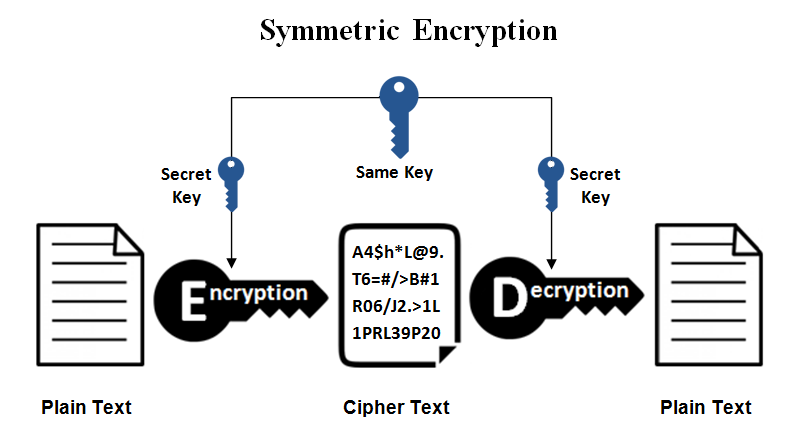
\includegraphics[width=0.6\textwidth]{sym} \\
\cite{3}
\\

Die symmetrischen Verfahren können in zwei Gruppen aufgeteilt werden, Stromchiffren und Blockchiffren. Mit Stromchiffren wird der Klartext Zeichen für Zeichen ver- und auch entschlüsselt. Bei Blockchiffren werden Zeichen des Texts in feste Blockgrössen eingeteilt, so dass mehrere Zeichen in einem Schritt ver- oder auch entschlüsselt werden können. \\

Bei der symmetrischen Verschlüsselung muss der Schlüssel gut geschützt werden da er direkten Zugriff auf die Daten gibt. Die grösste Gefahr für den Schlüssel ist in der Übermittlung. Aus diesem Grund gibt es spezielle Protokolle um dies zu machen. Das bekannteste Protokoll ist \href{https://www.youtube.com/watch?v=NmM9HA2MQGI}{Diffie-Hellman}. \\


\textbf{Vorteile:}
\begin{itemize}
    \item Einfaches Schlüsselmanagement, da nur ein Schlüssel für Ent- und Verschlüsselung benötigt wird
    \item Hohe Geschwindigkeit für Ent- und Verschlüsselung, da Verfahren meist auf effizienten Operationen wie Bit-Shifts und XORs aufbauen
\end{itemize}\cite{1} \\

\textbf{Nachteile:}
\begin{itemize}
    \item Nur ein Schlüssel für Ver- und Entschlüsselung, Schlüssel darf nicht in unbefugte Hände gelangen
    \item Schlüssel muss über einen sicheren Weg übermittelt werden
    \item Anzahl der Schlüssel bezogen auf die Anzahl der Teilnehmer wächst quadratisch
\end{itemize}\cite{1} \\

\section*{Asymmetrische Verschlüsselung}

Bei einem Asymmetrischen Verschlüsselungsverfahren werden zwei Schlüssel verwendet zum ver- und entschlüsseln. Dieses sogenannte Schlüsselpaar setzt sich aus einem privaten Schlüssel und einem öffentlichen Schlüssel zusammen. Mit dem privaten Schlüssel, werden Daten Entschlüsselt oder eine digitale Signatur erzeugt. Mit dem öffentlichen Schlüssel kann man Daten verschlüsseln und erzeugte Signaturen auf ihre Authentizität überprüfen. \\

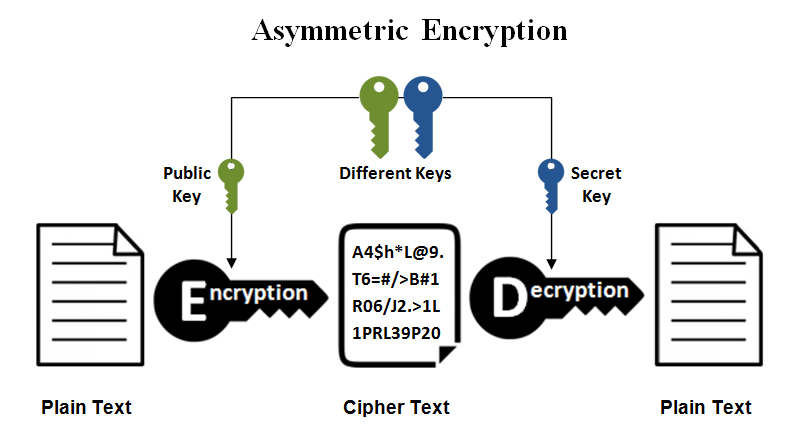
\includegraphics[width=0.6\textwidth]{asym.png} \\
\cite{4} \\

\textbf{Asymmetrische Kryptosysteme:}
\begin{itemize}
    \item Ed25519, Ed448 signing
    \item X25519, X448 key exchange
    \item Elliptic curve cryptography
    \item RSA
    \item Diffie-Hellman key exchange
    \item DSA
    \item Key Serialization
    \item Asymmetric Utilities
\end{itemize}
\cite{2} \\

Am Anfang wird der öffentliche Schlüssel veröffentlicht. Es gibt viele wege um einen Schlüssel zu veröffentlichen, es gibt sogar Server die auf darauf spezialisiert sind. Jeder der den öffentlichen Schlüssel hat kann jetzt Nachrichten verschlüsseln oder eine Signierte Nachricht verifizieren. \\

Der private Schlüssel muss um jeden Preis geheim halten werden, da die Daten nur damit entschlüsselt werden können. Mit dem privaten Schlüssel können die verschlüsselten Daten entschlüsselt werden und Nachrichten signiert werden.\\

Zu beachten ist bei der Verschlüsselung, dass je nach verwendetem Schlüssel bei der Verschlüsselung derselben Daten unterschiedliche verschlüsselte Daten entstehen können. \cite{2} \\


Anwendung finden asymmetrische Kryptosysteme bei Verschlüsselungen, Authentifizierungen und der Sicherung der Integrität. Bekannte Beispiele die auf asymmetrische Verfahren aufbauen sind OpenPGP oder auchS/MIME. Aber auch kryptografische Protokolle wie SSH, SSL/TLS oder auch https bauen auf asymmetrische Kryptosysteme. Weiter Anwendung findet bei digitalen Signaturen statt.\cite{2} \\

\textbf{Vorteile:}
\begin{itemize}
    \item Relativ Hohe Sicherheit
    \item Es werden nicht so viele Schlüssel benötigt wie bei einem symmetrischen Verschlüsselungsverfahren, somit weniger Aufwand der Geheimhaltung des Schlüssels
    \item Kein Schlüsselverteilungsproblem, da Public Key für jeden ohne Probleme zu erreichen ist
    \item Möglichkeit der Authentifikation durch elektronische Unterschriften (digitale Signaturen)
\end{itemize}
\cite{2} \\

\textbf{Nachteile:}
\begin{itemize}
    \item Asymmetrischen Algorithmen arbeiten sehr langsam ca. 10 000 Mal langsamer als symmetrische.
    \item Große benötigte Schlüssellänge
    \item Probleme bei mehreren Empfänger einer verschlüsselten Nachricht, da jedes Mal die Nachricht extra verschlüsselt werden muss. Abhilfe schaffen hybride Verfahren
    \item Sicherheitsrisiko durch für jeden zugänglichen Public Key, Man in the Middle
\end{itemize}
\cite{2}

\begin{thebibliography}{9}
    \bibitem[Kryptowissen 1]{1} \emph{\url{https://www.kryptowissen.de/symmetrische-verschluesselung.html}}, used: 28.03.2020
    \bibitem[Kryptowissen 2]{2} \emph{\url{https://www.kryptowissen.de/asymmetrische-verschluesselung.html}}, used: 28.03.2020
    \bibitem[ssl2buy]{3} \emph{\url{https://www.ssl2buy.com/wiki/wp-content/uploads/2015/12/Symmetric-Encryption.png}}, used: 03.04.2020
    \bibitem[ssl2buy]{4} \emph{\url{https://www.ssl2buy.com/wiki/wp-content/uploads/2015/12/Asymmetric-Encryption.png}}, used: 03.04.2020
\end{thebibliography}
\end{document}